\documentclass[tikz,border=12pt]{standalone}
\usepackage[T1]{fontenc}
\usepackage{mathpazo}
\usepackage{amsmath,amssymb}
\usetikzlibrary{arrows.meta, positioning, calc}

\definecolor{stblue}{HTML}{7B97AD}
\definecolor{rwgold}{HTML}{B8995E}
\definecolor{sage}{HTML}{7A9A7E}
\definecolor{dkbrown}{HTML}{3D3530}
\definecolor{wmgray}{HTML}{7B7067}
\definecolor{cream}{HTML}{F9F6F0}
\definecolor{border}{HTML}{D4C9B8}
\definecolor{terracotta}{HTML}{C47A6A}

\begin{document}
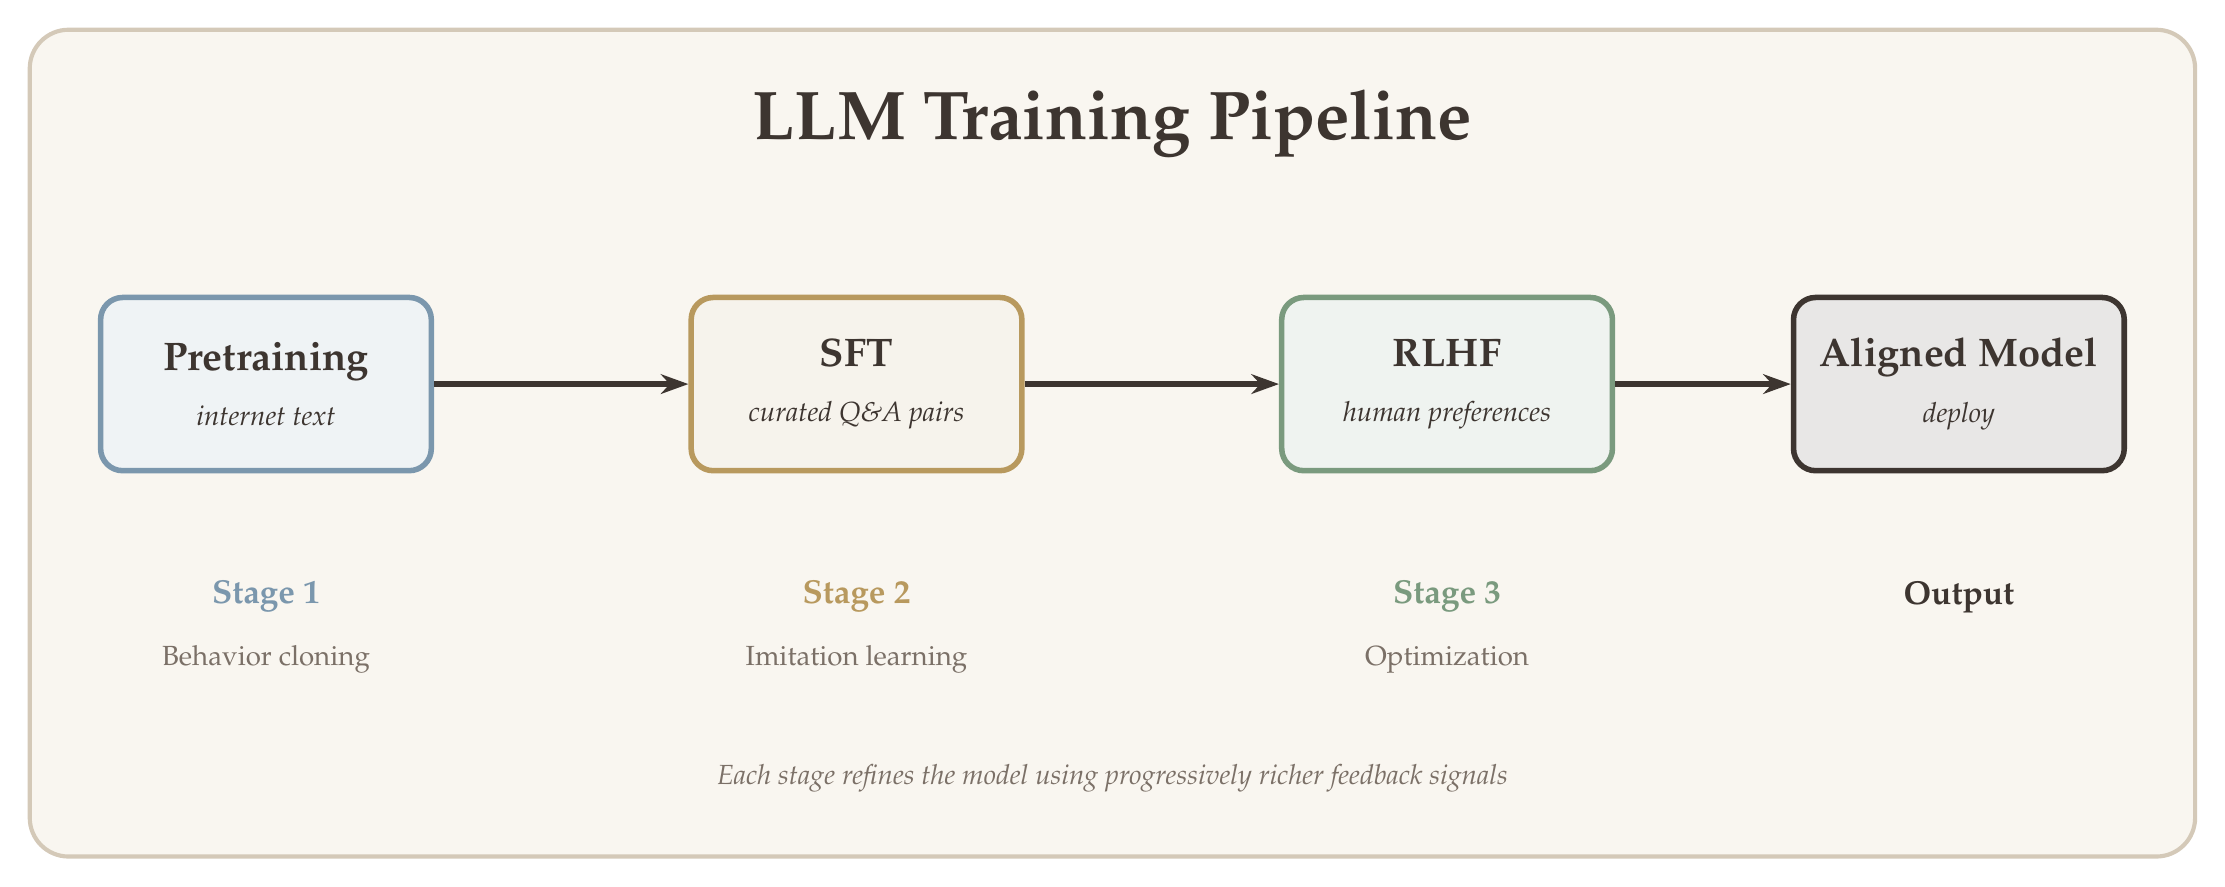
\begin{tikzpicture}[
  >={Stealth[length=3.5mm, width=2.5mm]},
  pbox/.style={
    draw=#1, line width=2pt, fill=#1!12, rounded corners=8pt,
    minimum width=42mm, minimum height=22mm, font=\Large\bfseries, text=dkbrown,
    align=center, inner sep=6pt
  },
  arr/.style={->, line width=2pt, dkbrown},
  stlbl/.style={font=\large, align=center},
]

% Background
\fill[cream, rounded corners=14pt] (-1.5,-4.5) rectangle (26,6);
\draw[border, rounded corners=14pt, line width=1.5pt] (-1.5,-4.5) rectangle (26,6);

% Title
\node[font=\Huge\bfseries, text=dkbrown] at (12.25,4.8)
  {LLM Training Pipeline};

% Four pipeline boxes
\node[pbox=stblue] (pretrain) at (1.5,1.5)
  {Pretraining\\[2pt]
   {\normalsize\mdseries\textit{internet text}}};

\node[pbox=rwgold] (sft) at (9,1.5)
  {SFT\\[2pt]
   {\normalsize\mdseries\textit{curated Q\&A pairs}}};

\node[pbox=sage] (rlhf) at (16.5,1.5)
  {RLHF\\[2pt]
   {\normalsize\mdseries\textit{human preferences}}};

\node[pbox=dkbrown] (aligned) at (23,1.5)
  {Aligned Model\\[2pt]
   {\normalsize\mdseries\textit{deploy}}};

% Arrows
\draw[arr] (pretrain.east) -- (sft.west);
\draw[arr] (sft.east) -- (rlhf.west);
\draw[arr] (rlhf.east) -- (aligned.west);

% Stage labels below
\node[stlbl, text=stblue, font=\large\bfseries] at (1.5,-1.2) {Stage 1};
\node[stlbl, text=wmgray, font=\normalsize] at (1.5,-2) {Behavior cloning};

\node[stlbl, text=rwgold, font=\large\bfseries] at (9,-1.2) {Stage 2};
\node[stlbl, text=wmgray, font=\normalsize] at (9,-2) {Imitation learning};

\node[stlbl, text=sage, font=\large\bfseries] at (16.5,-1.2) {Stage 3};
\node[stlbl, text=wmgray, font=\normalsize] at (16.5,-2) {Optimization};

\node[stlbl, text=dkbrown, font=\large\bfseries] at (23,-1.2) {Output};

% Bottom annotation
\node[font=\normalsize\itshape, text=wmgray] at (12.25,-3.5)
  {Each stage refines the model using progressively richer feedback signals};

\end{tikzpicture}
\end{document}
